% ===========================================================================
% 附录 AP：维护与遥操作——从热室到包层更换
% ---------------------------------------------------------------------------
% 数值唯一来源：tools/calc/appAP_calc.py -> tools/calc/appAP_calc.txt
%   重生成：python tools\calc\appAP_calc.py | Out-File -Encoding utf8 tools\calc\appAP_calc.txt
%   正文里凡标出数字的量都必须能在这个输出里找到；改数字先改脚本。
% 工作点：与附录 Z / AJ / AK / AO 同一台（P_fus = 556.5 MW），
%   电厂侧声明量：P_e = 200 MW、电价 0.4 元/kWh、年 8760 h。
% 单位口径：数字与单位一起进数学模式（$1920\ \mathrm{h}$）；
%   中文只能进 \text{}，绝不允许写进 \mathrm{}（否则编译会缺字形）；
%   无量纲比值一律写成小数，并在括号里给出百分数。
% 版权口径：只借鉴结论、量级与题型，不复制任何教材的原文、图、表或习题；
%   每节末尾注明出处（书名/作者/年份/卷期页）。
% 这一篇讲什么：
%   Z 讲聚变堆工程（包层、氚循环与电厂账），AK 讲安全与环境（氚与废物分级），
%   AO 讲真空与壁处理（抽速、放气与壁上库存），AM 讲磁体与超导。
%   本附录只回答一件事：\textbf{这些东西坏了、到寿命了，怎么换}——
%   可用因子、冷却窗口、遥操作精度、热室流转与人因剂量预算。
% ===========================================================================

\section{为什么维护是一门物理课：可用因子}
\label{sec:app-ap-availability}

一台聚变堆能不能发电，最终不是由等离子体物理单独决定的，而是由
「它一年能运行多少小时」决定的。把这个小时数写成比值，就是\textbf{可用因子}：

\begin{equation}
A = 1 - \frac{t_{\text{down}}}{t_{\text{year}}},
\label{eq:app-ap-avail}
\end{equation}

其中 $t_{\text{year}} = 8760\ \mathrm{h}$，$t_{\text{down}}$ 是一年里所有停机小时数之和。
本书的工作点取计划维护 $60\ \mathrm{d}$、非计划停机 $20\ \mathrm{d}$，于是
$t_{\text{down}} = 1920\ \mathrm{h}$、$A = 0.780822$——也就是说，
\textbf{五分之一的发电能力在设计阶段就被停机吃掉了}。

停机不是「少发一点电」，而是直接少一笔钱。声明净电功率 $P_e = 200\ \mathrm{MW}$、
电价 $0.4$ 元$/\mathrm{kWh}$，停机损失可以写成一次乘法：

\begin{equation}
C_{\text{lost}} = P_e\, t_{\text{down}}\, p,
\label{eq:app-ap-cost}
\end{equation}

代入得 $C_{\text{lost}} = 1.536\times10^{8}$ 元，即\textbf{每停机一天损失
$1.92\times10^{6}$ 元}；全年满发是 $1.752\times10^{6}\ \mathrm{MWh}$，
停机拿走的份额正是 $0.219178$。

\begin{table}[htbp]
\centering
\small
\caption{停机账：可用因子与代价（$P_e = 200\ \mathrm{MW}$，电价 $0.4$ 元$/\mathrm{kWh}$）}
\label{tab:app-ap-avail}
\setlength{\tabcolsep}{4pt}
\begin{tabular}{p{5.6cm}p{4.4cm}p{5.6cm}}
\toprule
项目 & 数值 & 说明 \\
\midrule
计划维护 & $60\ \mathrm{d}$ & 包层/偏滤器更换、烘烤、检查 \\
非计划停机 & $20\ \mathrm{d}$ & 故障与修复（设计指标） \\
停机小时 & $1920\ \mathrm{h}$ & 两项之和 \\
可用因子 & $0.780822$ & 全年可发电小时份额 \\
停机的发电量损失 & $384000\ \mathrm{MWh}$ & $P_e \times t_{\text{down}}$ \\
停机的售电损失 & $1.536\times10^{8}$ 元 & 按上述电价 \\
每停机一天的损失 & $1.92\times10^{6}$ 元$/$天 & 停机成本的时间单价 \\
\bottomrule
\end{tabular}
\end{table}

\begin{tip}{可用因子是设计指标，不是运维指标}{tip-app-ap-avail}
可用因子在图纸阶段就被三件事定死了：包层能撑几年、冷却要等多久、热室一年能周转几段。
运行阶段能做的只是别把这三件事弄得更糟。所以本附录的顺序是
\textbf{寿命 $\rightarrow$ 冷却 $\rightarrow$ 遥操作 $\rightarrow$ 热室 $\rightarrow$ 人因}，
而不是反过来。
\end{tip}

{\footnotesize
\textbf{出处：}维护与可用性的工程口径参照 Dolan（编）\textit{Magnetic Fusion Technology}
（2013）第 15 章「维护与远程处理」、Wesson \textit{Tokamaks} 4th ed.（2011）第 1 章
对装置运行窗口的讨论。
}

\section{包层寿命与更换周期}
\label{sec:app-ap-blanket}

包层是消耗品。中子把它加热、把它活化、也把它的结构原子撞离格点
（这部分账在附录 AK 里算过：$4.5472\ \mathrm{dpa}/$年，$10.996$ 年累计 $50.001\ \mathrm{dpa}$）。
工程上不会等到它坏，而是按一个\textbf{更换周期}去换。声明包层总质量
$M = 1.0\times10^{6}\ \mathrm{kg}$、分成 $N = 16$ 个扇形段，则单段质量

\begin{equation}
m_{\text{sec}} = \frac{M}{N} = 62500\ \mathrm{kg} = 62.5\ \mathrm{t}.
\label{eq:app-ap-sector}
\end{equation}

声明更换周期 $T_{\text{blanket}} = 5$ 年、电厂寿命 $T_{\text{plant}} = 40$ 年，则

\begin{equation}
n_{\text{change}} = \frac{T_{\text{plant}}}{T_{\text{blanket}}} = 8\ \text{次},
\qquad
\dot n = \frac{n_{\text{change}} N}{T_{\text{plant}}} = 3.2\ \text{段}/\text{年}.
\label{eq:app-ap-campaign}
\end{equation}

平均每年 $3.2$ 段、每段 $62.5\ \mathrm{t}$，就是 $200\ \mathrm{t}/$年 的更换量。
把它摊到每年的停机小时上，每段平均只有 $600\ \mathrm{h}$——不到四天。
\textbf{维护设计的第一条约束就出现了：更换工期的量级必须按「天」算，不能按「周」算。}

\begin{table}[htbp]
\centering
\small
\caption{包层更换的规模账（$M = 1.0\times10^{6}\ \mathrm{kg}$，$N = 16$，寿命 $40$ 年）}
\label{tab:app-ap-blanket}
\setlength{\tabcolsep}{4pt}
\begin{tabular}{p{5.6cm}p{4.4cm}p{5.6cm}}
\toprule
项目 & 数值 & 说明 \\
\midrule
单个扇形段质量 & $62500\ \mathrm{kg}$ & $= 62.5\ \mathrm{t}$ \\
全寿期更换次数 & $8$ & 40 年 $/$ 5 年 \\
全寿期更换段数 & $128$ & 每次 16 段 \\
平均每年更换段数 & $3.2$ & 128 段 $/$ 40 年 \\
平均每年更换质量 & $200\ \mathrm{t}$ & $3.2 \times 62.5$ \\
每段可用工期 & $600\ \mathrm{h}$ & 1920 h $/$ 3.2 段 \\
\bottomrule
\end{tabular}
\end{table}

\begin{tip}{更换周期是设计输入，不是寿命预测}{tip-app-ap-blanket}
$5$ 年不是「材料五岁会坏」，而是「我们决定每五年换一次，好让后面的账都能算」。
周期定得短，可用因子被停机吃掉；定得长，包层在中子剂量下先坏。
真正的寿命由 \textbf{dpa 与氦脆}决定（附录 AK），周期只是人为选定的整数。
\end{tip}

{\footnotesize
\textbf{出处：}包层与增殖段维护的工程口径参照 ITER Physics Basis
（\textit{Nuclear Fusion} \textbf{39}, 1999）第 4 章、Dolan（编）
\textit{Magnetic Fusion Technology}（2013）第 6 章与第 15 章。
}

\section{活化与冷却窗口：剂量率的两个分量}
\label{sec:app-ap-dose}

换包层之前要先「等」。停堆 1 天后现场剂量率声明为
$10^{4}\ \mathrm{Sv}/\mathrm{h}$（短寿命活化产物主导），此外还有一个几乎不衰减的长寿命分量
$10\ \mathrm{mSv}/\mathrm{h}$（Co-60 主导，半衰期 $5.2711$ 年，与附录 AK 同口径）。
两个分量叠起来：

\begin{equation}
D(t) = D_{\text{long}} + D_0\,2^{-t/T_{\text{short}}},
\label{eq:app-ap-decay}
\end{equation}

其中 $D_0 = 10^{4}\ \mathrm{Sv}/\mathrm{h}$、$T_{\text{short}} = 2.5\ \mathrm{d}$。
要让剂量率降到远程操作阈值 $D_{\text{remote}} = 1\ \mathrm{Sv}/\mathrm{h}$，解出冷却时间

\begin{equation}
t_{\text{cool}} = T_{\text{short}}\log_2\frac{D_0}{D_{\text{remote}} - D_{\text{long}}}
= 33.2555\ \mathrm{d},
\label{eq:app-ap-cooling}
\end{equation}

降到 $0.1\ \mathrm{Sv}/\mathrm{h}$ 则要 $41.9041\ \mathrm{d}$。
注意分母里那个减号：长寿命分量决定了\textbf{冷却时间的上限}——
当目标低于 $D_{\text{long}}$ 时，等多久都没用。

这正是人工进入的问题所在。人工阈值取 $10\ \mu\mathrm{Sv}/\mathrm{h}$，
它比长寿命分量小三个数量级，于是

\begin{equation}
t_{\text{hands}} = T_{\text{long}}\log_2\frac{D_{\text{long}}}{D_{\text{hands}}}
= 52.5306\ \text{年}.
\label{eq:app-ap-hands}
\end{equation}

\textbf{停堆半个世纪以后，人才可以不带屏蔽地站到包层前面。}这句话等价于：
聚变堆的维护必须是遥操作，没有第二条路。

工期内的累积剂量是式~\eqref{eq:app-ap-decay} 的积分。从第 $33.2555$ 天起、
按 $30\ \mathrm{d}$ 工期算，未屏蔽累积 $10.7698\ \mathrm{Sv}$；
乘上屏蔽因子 $10^{-4}$ 后是 $1.07698\times10^{-3}\ \mathrm{Sv}$，即
\textbf{只占器件耐总剂量（$10^{5}\ \mathrm{Gy}$）的 $1.07698\times10^{-8}$}。

\begin{equation}
\mathcal{D}_{\text{acc}} = D_{\text{long}}\,t_{\text{turn}}
+ \frac{D_0 T_{\text{short}}}{\ln 2}
\left(2^{-t_0/T_{\text{short}}} - 2^{-t_1/T_{\text{short}}}\right),
\label{eq:app-ap-acc}
\end{equation}

\begin{equation}
\mathcal{D}_{\text{shield}} = f_{\text{shield}}\,\mathcal{D}_{\text{acc}}.
\label{eq:app-ap-shield}
\end{equation}

\begin{table}[htbp]
\centering
\small
\caption{冷却窗口与累积剂量（$D_0 = 10^{4}\ \mathrm{Sv}/\mathrm{h}$，$T_{\text{short}} = 2.5\ \mathrm{d}$，$D_{\text{long}} = 10\ \mathrm{mSv}/\mathrm{h}$）}
\label{tab:app-ap-dose}
\setlength{\tabcolsep}{4pt}
\begin{tabular}{p{5.8cm}p{4.2cm}p{5.6cm}}
\toprule
项目 & 数值 & 说明 \\
\midrule
降到 $1\ \mathrm{Sv}/\mathrm{h}$ & $33.2555\ \mathrm{d}$ & 远程操作开工线 \\
降到 $0.1\ \mathrm{Sv}/\mathrm{h}$ & $41.9041\ \mathrm{d}$ & 进一步保守 \\
一年后的剂量率 & $0.01\ \mathrm{Sv}/\mathrm{h}$ & 短寿命分量已消失 \\
十年后的剂量率 & $2.68476\times10^{-3}\ \mathrm{Sv}/\mathrm{h}$ & 仍远高于人工阈值 \\
降到 $10\ \mu\mathrm{Sv}/\mathrm{h}$ & $52.5306$ 年 & 人工进入不可行 \\
30 天累计（未屏蔽） & $10.7698\ \mathrm{Sv}$ & 从开工线起算 \\
30 天累计（屏蔽后） & $1.07698\times10^{-3}\ \mathrm{Sv}$ & $f_{\text{shield}} = 10^{-4}$ \\
占器件耐总剂量 & $1.07698\times10^{-8}$ & 器件寿命不由辐照决定 \\
\bottomrule
\end{tabular}
\end{table}

\begin{tip}{剂量率有两个分量，它们管两件不同的事}{tip-app-ap-dose}
短寿命分量决定「等多久能开工」（$33.2555$ 天）；长寿命分量决定「人工永远不行」（$52.5306$ 年）。
把两者混成一个「半衰期」是维护分析里最常见的错误——一个会低估冷却时间，
另一个会高估屏蔽需求。
\end{tip}

{\footnotesize
\textbf{出处：}活化与剂量率的工程口径参照 Gilbert 与 Sublet 的活化计算综述
（2010 年代）。
Turner \textit{Atoms, Radiation, and Radiation Protection}
（2007）。
ICRP 第 103 号报告（2007）的剂量限值框架。
}

\begin{figure}[htbp]
\centering
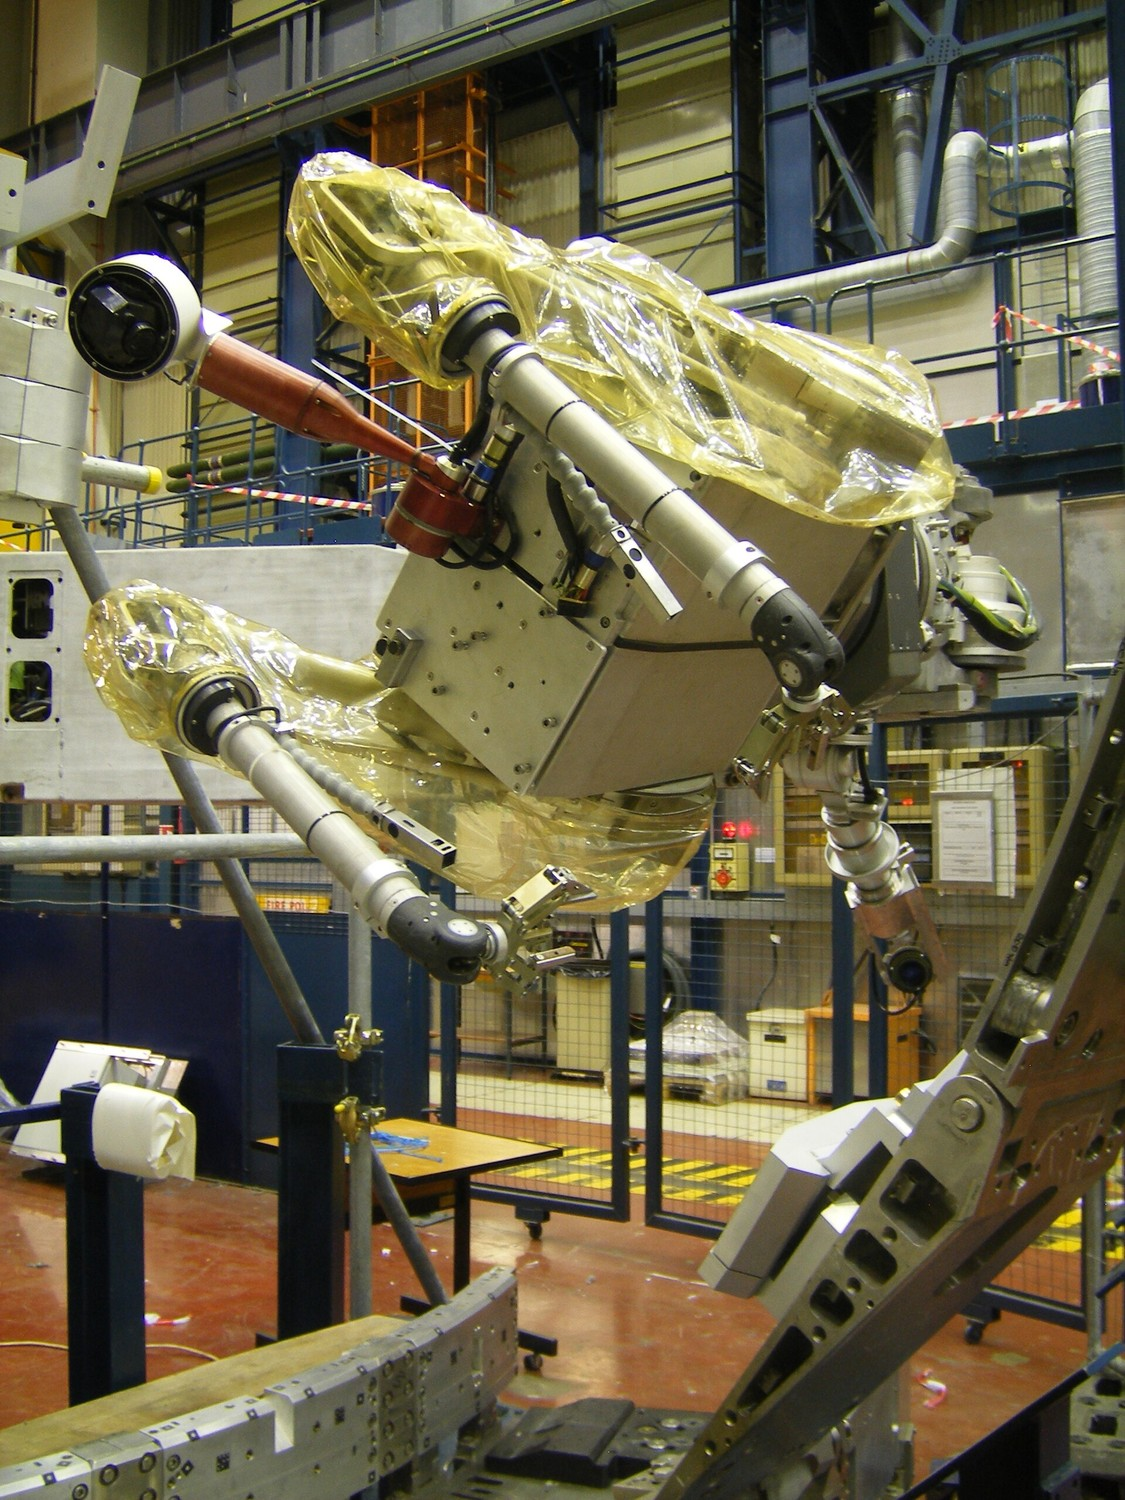
\includegraphics[width=0.67\textwidth]{../figures/jet_mascot.jpg}
\caption{遥操作的真实尺度：JET 的机械臂。聚变装置的遥操作不是「远程看视频」：机械臂要在狭窄空间里完成毫米级定位、带着力反馈、还要容忍信号延迟——本章遥操作那一节的三个约束都在这里。}
\label{fig:photo-appap}
\figsource{Steve Parker from Ash Vale, UK，CC BY 2.0（Wikimedia Commons），链接见 figures/CREDITS.md。}
\end{figure}

\section{遥操作：精度、力反馈与延迟}
\label{sec:app-ap-teleop}

既然人工进入要等半个世纪，切割、吊装、对中、焊接就都得由机器完成。
机械臂的臂端定位误差可以写成一次乘法：

\begin{equation}
e = L\,\varepsilon,
\label{eq:app-ap-err}
\end{equation}

声明臂长 $L = 5\ \mathrm{m}$、相对精度 $\varepsilon = 0.2\ \mathrm{mm}/\mathrm{m}$，
得 $e = 0.001\ \mathrm{m}$，也就是 \textbf{$1\ \mathrm{mm}$}。而包层段的装配间隙取
$0.5\ \mathrm{mm}$，余量

\begin{equation}
\frac{\delta}{e} = 0.5
\label{eq:app-ap-margin}
\end{equation}

——\textbf{小于 1}。这句话的意思是：单靠臂的绝对精度装不上，必须靠局部视觉伺服或导向销
把误差在最后几厘米里再吃掉一次。这是遥操作设计的第一个真结论。

力反馈的分辨率同样是一次比值：声明力传感器分辨率 $0.1\ \mathrm{N}$、
插拔力 $100\ \mathrm{N}$，则

\begin{equation}
\frac{\Delta F}{F} = \frac{0.1}{100} = 0.001.
\label{eq:app-ap-force}
\end{equation}

$0.1\%$ 的力分辨率足以「摸到」卡涩，但不足以判断焊缝是否熔透——所以焊接仍要
靠电参数与视觉，而不是靠手感。最后是延迟：主从回路延迟声明 $100\ \mathrm{ms}$，
要在一个 $1\ \mathrm{cm}$ 的目标上不冲过头，操作速度上限

\begin{equation}
v_{\max} = \frac{0.01\ \mathrm{m}}{0.1\ \mathrm{s}} = 0.1\ \mathrm{m}/\mathrm{s},
\label{eq:app-ap-latency}
\end{equation}

而 $10\ \mathrm{Hz}$ 的伺服带宽对应 $0.1\ \mathrm{s}$ 的周期——两个数字是同一件事的
两种写法：\textbf{延迟决定了「慢」是遥操作的物理属性，不是操作员手笨}。

\begin{table}[htbp]
\centering
\small
\caption{遥操作的关键指标（臂长 $5\ \mathrm{m}$，装配间隙 $0.5\ \mathrm{mm}$）}
\label{tab:app-ap-teleop}
\setlength{\tabcolsep}{4pt}
\begin{tabular}{p{5.8cm}p{4.2cm}p{5.6cm}}
\toprule
项目 & 数值 & 说明 \\
\midrule
臂端定位误差 & $0.001\ \mathrm{m}$ & $L\varepsilon$，即 $1\ \mathrm{mm}$ \\
相对装配间隙的余量 & $0.5$ & 小于 1，必须二次对中 \\
力反馈相对分辨率 & $0.001$ & $0.1\ \mathrm{N} / 100\ \mathrm{N}$ \\
延迟对应的速度上限 & $0.1\ \mathrm{m}/\mathrm{s}$ & $1\ \mathrm{cm} / 0.1\ \mathrm{s}$ \\
伺服带宽对应的周期 & $0.1\ \mathrm{s}$ & $1/10\ \mathrm{Hz}$ \\
\bottomrule
\end{tabular}
\end{table}

\begin{tip}{遥操作不是「远程看视频」}{tip-app-ap-teleop}
视频只提供视觉，而装配需要\textbf{力}。遥操作的核心是带力反馈的伺服回路：
位置由臂保证、最后的毫米由视觉与导向保证、手感由力传感器保证，
三者缺一不可。少了任何一项，工期就会从「天」变成「周」——而按
表~\ref{tab:app-ap-blanket}，每段只有 $600\ \mathrm{h}$。
\end{tip}

{\footnotesize
\textbf{出处：}遥操作与机器人学的工程口径参照 Siciliano 与 Khatib（编）
\textit{Springer Handbook of Robotics} 2nd ed.（2016）第 4 部分「现场与服务机器人」、
Dolan（编）\textit{Magnetic Fusion Technology}（2013）第 15 章。
}

\begin{figure}[htbp]
\centering
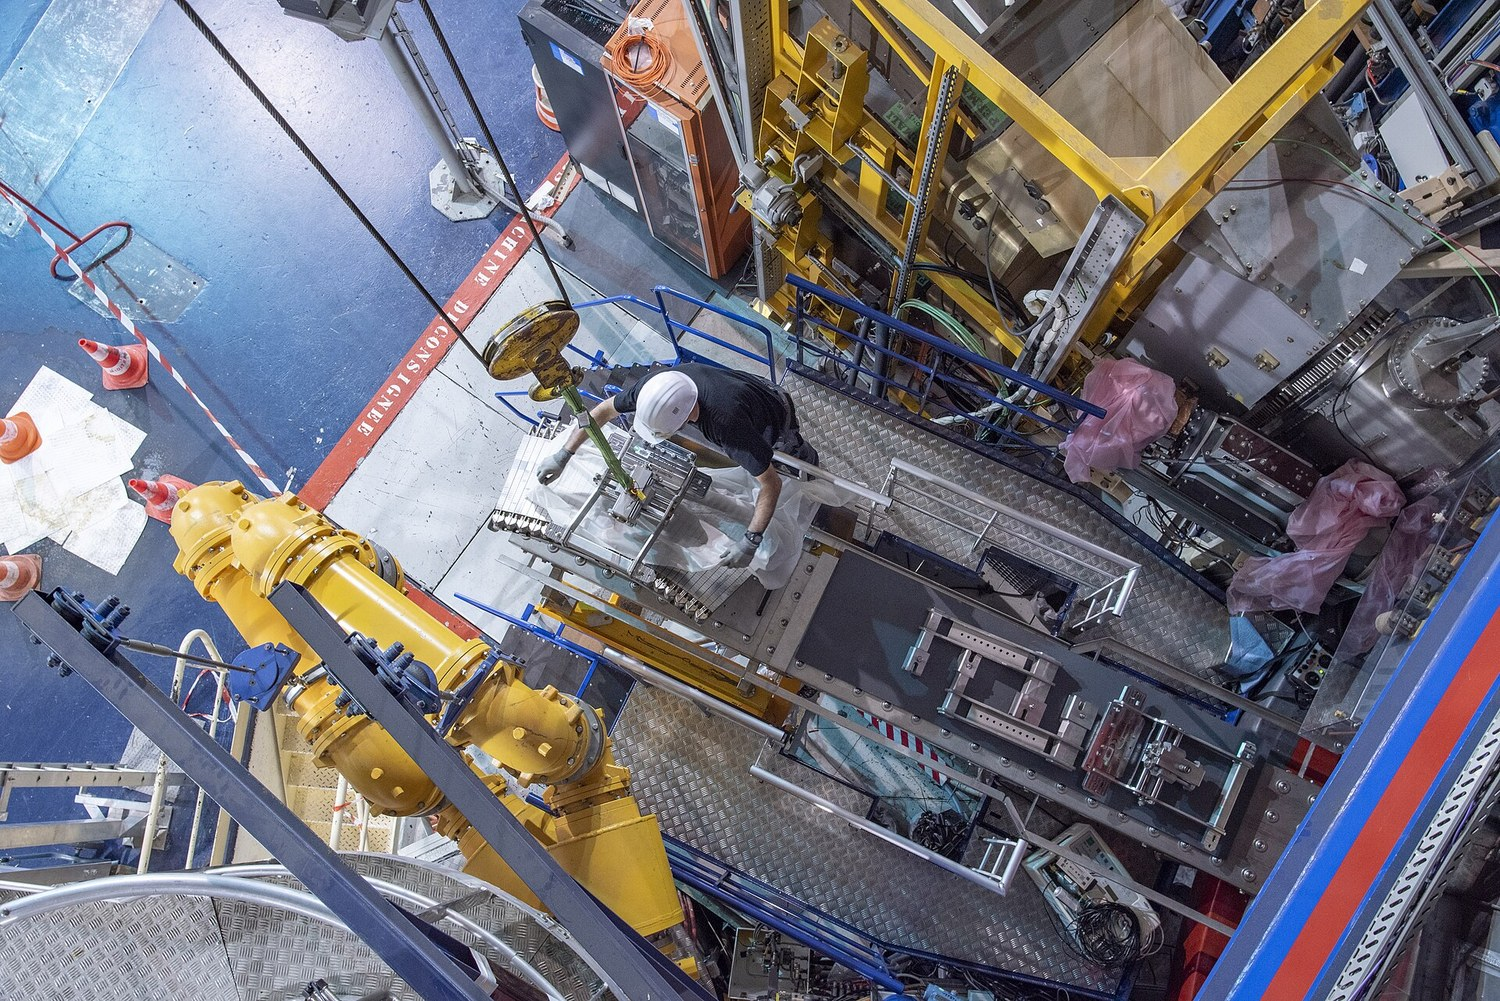
\includegraphics[width=0.78\textwidth]{../figures/ap_west_sector.jpg}
\caption{WEST 托卡马克在更换一个新扇区：整段真空室部件在厂房里装好、检漏，再用吊装与遥操作送到位。包层更换的时间与能力余量，就写在这种工序里。}
\label{fig:photo-appap3}
\figsource{Christophe Roux / IRFM，CC BY 4.0（Wikimedia Commons）}
\end{figure}

\section{热室与部件流转：能力余量}
\label{sec:app-ap-hotcell}

换下来的段是强放射源，不能就地拆——它要被装进屏蔽容器（cask）运到热室。
于是维护能力变成一道除法题。需求是

\begin{equation}
\dot n_{\text{need}} = \frac{n_{\text{change}}N}{T_{\text{plant}}} = 3.2\ \text{段}/\text{年},
\label{eq:app-ap-need}
\end{equation}

能力是「容器数 $\times$ 每容器年周转次数」：

\begin{equation}
\dot n_{\text{cap}} = \frac{N_{\text{cask}}\,365}{t_{\text{turn}}}
= \frac{2 \times 365}{30} = 24.3333\ \text{段}/\text{年},
\label{eq:app-ap-cap}
\end{equation}

余量

\begin{equation}
\frac{\dot n_{\text{cap}}}{\dot n_{\text{need}}} = 7.60417.
\label{eq:app-ap-capmargin}
\end{equation}

即 $7.60417$ 倍（$760.417\%$）的余量。看起来很宽，但两个 $30\ \mathrm{d}$ 的工位同时只占用
$0.263014$ 个——真正紧的不是容器，而是\textbf{热室工位与人员排班}：
单工位年周转 $12.1667$ 段，两个工位刚好覆盖需求并留出检修窗口。

\begin{table}[htbp]
\centering
\small
\caption{热室与 cask 流转账（$t_{\text{turn}} = 30\ \mathrm{d}$，2 个 cask，2 个工位）}
\label{tab:app-ap-hotcell}
\setlength{\tabcolsep}{4pt}
\begin{tabular}{p{5.8cm}p{4.2cm}p{5.6cm}}
\toprule
项目 & 数值 & 说明 \\
\midrule
年更换需求 & $3.2$ 段$/$年 & 与表~\ref{tab:app-ap-blanket} 同 \\
cask 年转运能力 & $24.3333$ 段$/$年 & $2 \times 365/30$ \\
能力余量 & $7.60417$ & 容器不是瓶颈 \\
单工位年周转能力 & $12.1667$ 段$/$年 & 真正的瓶颈 \\
同时占用工位数 & $0.263014$ & 平均在制段数 \\
\bottomrule
\end{tabular}
\end{table}

\begin{tip}{热室不是仓库，是工位}{tip-app-ap-hotcell}
把热室当仓库，就会按「能放几段」去设计；把它当工位，才会问
「一段要占多少天、同时能开几个工位、人手够不够」。
上表里容器余量 $7.6$ 倍而工位只能覆盖需求，就是这个区别。
\end{tip}

{\footnotesize
\textbf{出处：}热室与部件流转的口径参照 Dolan（编）\textit{Magnetic Fusion Technology}
（2013）第 15 章、IAEA 关于聚变装置远程处理与热室设施的公开技术文件（2000 年代）。
}

\section{在役检查与人因}
\label{sec:app-ap-human}

最后一道账是人。按剂量限值 $D_{\text{limit}} = 20\ \mathrm{mSv}/$年、
单次检修剂量 $D_{\text{inspect}} = 0.5\ \mathrm{mSv}$，一个人一年最多能进多少次：

\begin{equation}
N_{\text{allowed}} = \frac{D_{\text{limit}}}{D_{\text{inspect}}} = 40\ \text{次}/\text{年}.
\label{eq:app-ap-human}
\end{equation}

在役检查声明 $100$ 次$/$年、远程比例 $0.95$，则人工只剩 $5$ 次$/$年，
年剂量

\begin{equation}
D_{\text{year}} = N_{\text{hands}}D_{\text{inspect}} = 2.5\ \mathrm{mSv}/\text{年},
\label{eq:app-ap-budget}
\end{equation}

占限值的 $0.125$。反过来，远程次数是人工的

\begin{equation}
\frac{f_{\text{remote}}}{1 - f_{\text{remote}}} = 19\ \text{倍}.
\label{eq:app-ap-turns}
\end{equation}

\begin{table}[htbp]
\centering
\small
\caption{人因剂量预算（限值 $20\ \mathrm{mSv}/$年，单次 $0.5\ \mathrm{mSv}$）}
\label{tab:app-ap-human}
\setlength{\tabcolsep}{4pt}
\begin{tabular}{p{5.8cm}p{4.2cm}p{5.6cm}}
\toprule
项目 & 数值 & 说明 \\
\midrule
按单次剂量允许次数 & $40$ 次$/$年 & $20/0.5$ \\
在役检查的人工次数 & $5$ 次$/$年 & $100 \times 0.05$ \\
人工年剂量 & $2.5\ \mathrm{mSv}/$年 & $5 \times 0.5$ \\
占限值份额 & $0.125$ & 留出 $87.5\%$ 的余量 \\
远程相对人工次数倍数 & $19$ & $0.95/0.05$ \\
\bottomrule
\end{tabular}
\end{table}

\begin{tip}{剂量预算是乘出来的}{tip-app-ap-human}
「注意安全」不是指标，「每年多少次、每次多少毫西弗、总共占限值几成」才是。
把这三步写成式~\eqref{eq:app-ap-human}--\eqref{eq:app-ap-budget}，
预算就变成可以在设计阶段调整的数：原样能把限值压到 $12.5\%$，
就意味着还有余量去增加人工检查次数，或者把远程比例降到 $0.9$ 也不违规。
\end{tip}

{\footnotesize
\textbf{出处：}剂量限值与防护框架参照 ICRP 第 103 号报告（2007）。
Turner \textit{Atoms, Radiation, and Radiation Protection}（2007）。
}

\section{估算练习}
\label{sec:app-ap-problems}

\begin{enumerate}
\item \textbf{练习 1} 若把计划维护从 $60\ \mathrm{d}$ 压到 $45\ \mathrm{d}$，
非计划停机仍取 $20\ \mathrm{d}$，可用因子变成多少？比原来的方案提高多少？
\item \textbf{练习 2} 若包层更换周期从 $5$ 年缩短到 $3$ 年（同样的 $16$ 段），
平均每年要换多少段？是原来方案的几倍？
\item \textbf{练习 3} 若短寿命活化产物的半衰期只有 $1\ \mathrm{d}$（而不是 $2.5\ \mathrm{d}$），
降到 $1\ \mathrm{Sv}/\mathrm{h}$ 需要冷却多久？
\item \textbf{练习 4} 若屏蔽因子做到 $10^{-5}$（比正文更严十倍），
$30$ 天工期内的累积剂量是多少？占器件耐总剂量的几成？
\item \textbf{练习 5} 若把人工剂量限值按更保守的 $10\ \mathrm{mSv}/$年 计，
一个人一年最多能进几次（单次仍取 $0.5\ \mathrm{mSv}$）？
\item \textbf{练习 6} 若 cask 增加到 $4$ 个（周转时间不变），
年转运能力是多少？相对 $3.2$ 段$/$年 的需求有多大余量？
\end{enumerate}

\textbf{解答 1} $A = 1 - (45+20)\times24/8760 = 0.821918$，比 $0.780822$ 提高
$0.0410959$。也就是说省下 $15\ \mathrm{d}$ 的计划维护，能换回约 $4.10959\%$ 的发电时间。

\textbf{解答 2} 每年 $40/3 \times 16/40 = 5.33333$ 段，是 $5$ 年方案的 $1.66667$ 倍；
每年更换质量相应涨到 $333.333\ \mathrm{t}$（每段仍 $62.5\ \mathrm{t}$）。

\textbf{解答 3} 把 $T_{\text{short}} = 1\ \mathrm{d}$ 代入式~\eqref{eq:app-ap-cooling}，
得 $t_{\text{cool}} = 13.3022\ \mathrm{d}$——冷却窗口几乎缩短到原来的四成
（$13.3022/33.2555 = 0.4$），说明\textbf{短寿命核素的半衰期是维护工期的第一杠杆}。

\textbf{解答 4} $\mathcal{D}_{\text{shield}} = 10.7698 \times 10^{-5}
= 1.07698\times10^{-4}\ \mathrm{Sv}$，占器件耐总剂量的 $1.07698\times10^{-9}$。
再小一个数量级也还是远低于器件上限——辐照从来不是远程设备的寿命瓶颈，
可靠性与可维修性才是。

\textbf{解答 5} $N_{\text{allowed}} = 10/0.5 = 20$ 次$/$年，
正好是 $20\ \mathrm{mSv}$ 方案的一半。若仍要保持 $5$ 次人工检查，
年剂量 $2.5\ \mathrm{mSv}$ 只占新限值的 $0.25$，依然安全。

\textbf{解答 6} $\dot n_{\text{cap}} = 4 \times 365/30 = 48.6667$ 段$/$年，
余量 $48.6667/3.2 = 15.2083$。容器永远不是瓶颈——
真正的约束是热室工位与人员（表~\ref{tab:app-ap-hotcell}）。

\section{来源、分级与版权说明}
\label{sec:app-ap-source}

\begingroup\small
本附录的主题是\textbf{「机器坏了怎么换」}，因此它引用的是工程手册、
安全报告与机器人学教材，而不是等离子体物理的经典论文。
表~\ref{tab:app-ap-source} 列出借鉴来源与借鉴方式（只借鉴结论、量级与题型，
不复制原文、图表与习题）。

\begin{table}[htbp]
\centering
\small
\caption{本附录的借鉴来源与借鉴方式}
\label{tab:app-ap-source}
\setlength{\tabcolsep}{4pt}
\begin{tabular}{p{5.2cm}p{3.4cm}p{6.4cm}}
\toprule
来源 & 类型 & 借鉴内容 \\
\midrule
Dolan（编）\textit{Magnetic Fusion Technology}（2013） & 工程手册 & 可用因子、
维护与远程处理的工程口径 \\
Wesson \textit{Tokamaks} 4th ed.（2011） & 教材 & 装置运行窗口与停机代价的背景 \\
ITER Physics Basis，\textit{Nuclear Fusion} \textbf{39}（1999） & 设计报告 &
包层/偏滤器更换与维护方案 \\
Siciliano 与 Khatib（编）\textit{Springer Handbook of Robotics} 2nd ed.（2016） &
教材 & 遥操作、力反馈与延迟的工程判据 \\
ICRP 第 103 号报告（2007） & 安全标准 & 剂量限值与防护框架 \\
Turner \textit{Atoms, Radiation, and Radiation Protection}（2007） &
教材 & 剂量、屏蔽与累积剂量的算法 \\
Gilbert 与 Sublet 活化计算综述（2010 年代） & 综述 & 活化与剂量率的量级 \\
IAEA 远程处理与热室技术文件（2000 年代） & 技术文件 & cask 与热室流转口径 \\
\bottomrule
\end{tabular}
\end{table}

\begin{tip}{本附录没有涵盖什么}{tip-app-ap-honest}
这一篇不展开具体装置的维护方案、工期网络图与可靠性数据库，
也不给任何安全分析结论。它只做一件事：把「换一次包层」拆成
可用因子、冷却窗口、遥操作精度、热室流转、人因预算五笔可以用初中算术验证的账，
让读者在任何一台装置上都能量出自己的数。
\end{tip}

\textbf{不复制}本附录不复制上述来源的原文、图表、参数表与习题；
所有数值均由 \texttt{tools/\allowbreak{}calc/\allowbreak{}appAP\_calc.py} 按本附录声明的输入复算，
读者可以用同一脚本改输入重算。
\textbf{不复制}IEC/IAEA 标准文本与 ICRP 报告条文；
本附录只使用「$20\ \mathrm{mSv}/$年 与 $1\ \mathrm{mSv}/$年 这类限值数字」
作为预算的边界条件。
\textbf{不复制}任何厂商的遥操作机械臂规格表；
臂长、精度、力分辨率与延迟均为本附录自行声明的量级。
\textbf{不复制}具体热室设施的设计图与转运流程；
$30\ \mathrm{d}$ 周转与 $2$ 个 cask 是本附录为说明「除法题」而设的假设。
\endgroup
